\documentclass [a4paper,12pt]{article}
\usepackage[left = 2.5cm, rigth = 2.5cm, top = 3cm, bottom = 3 cm] {geometry}
\usepackage{amsmath,amsthm,amssymb}
\usepackage{cite}
\usepackage{url}
\usepackage[utf8]{inputenc}
\usepackage[spanish]{babel}
\usepackage{graphicx}
\bibliographystyle{plain}

\begin{document}
\title{Informe Moogle!}
\author{Abel Ponce Gonzalez}
\date{Julio, 2023}
\maketitle
\newpage
\tableofcontents
\newpage
\begin {abstract}
El artículo analiza el funcionamiento de un motor de búsqueda y sus desafíos. Se hace énfasis en las clases, propiedades de estas y métodos que se utilizaron para lograr el resultado final del proyecto, un buscador inteligente basado principalmente en Álgebra Lineal. 
\end{abstract}
\newpage
\section{Introducción}\label{sec:intro}
En este proyecto implemente una clase llamada documentos donde estaría la mayor parte del algoritmo, a la cual le di propiedades entre ellas están: archivos (posee las rutas de cada txt de la base datos), textos (posee cada texto de la base sin signos de puntuación), palabrasUnicas (lista de todas las palabras sin repetir), matriz (matriz numérica de TF-IDF). Ahora paso a paso iré explicando la implementación de los métodos para obtener las características de estas propiedades.
\newpage
\section{Desarrollo}\label{sec: ent}
\subsection{Propiedad \texttt{archivos}}\label{sub:center}
El buscador trabaja con una base de datos que implementaremos nosotros, así que lo primero que tenemos que hacer es buscar la forma de acceder a estos documentos y hacer de esto un método dinámico y la forma que encontré fue a través de la clase Directory y el método de esta clase GetCurrentDirector.
\subsection{Propiedad \texttt{textos}}\label{sub:center}
Esta propiedad la hice a partir del método Documento, que a través de las rutas obtenidas por la propiedad archivos y utilizando la clase File consigo los textos de cada uno de los términos dentro del array archivos. Luego utilizando el método Replace y ToLower elimino los signos de puntuación de los textos y los pongo en minúscula para trabajar mucho más fácil con ellos (en el método QuitarPuntuacion). 
\subsection{Propiedad \texttt{palabrasUnicas}}\label{sub:center}
Mi próximo paso fue crear una lista que contuviera todas las palabras de todos los documentos sin repetir para que fuera más sencillo el cálculo de TF-IDF que más adelante explicaré. La creación de esta lista fue bastante sencilla ya que solo me tuve que apoyar en la clase HashSet que gracias a su funcionalidad de no tomar palabras que ya contiene hice mucho más efectivo el método. Para obtener las palabras de cada texto utilizaba ya la propiedad creada textos e iba guardando cada palabra de él en un array de string utilizando el método Split. Luego iba añadiendo a la HashSet.
\subsection{Propiedad \texttt{matriz}}\label{sub:center}
 La idea para la creación de mi matriz es que las columnas van a representar las palabras y las filas los documentos entonces cada término de la matriz va a ser el valor de TF-IDF de una palabra en un documento. EL objetivo de rellenar esta matriz con los valores de TF-IDF es que de esta manera estamos haciendo cada documento(filas) un vector a partir de la lista de palabras únicas.
\subsection{Propiedad \texttt{TF-IDF}}\label{sub:center}
Lo necesario para hallar el TF-IDF es primero hallar el TF que no es más que la frecuencia bruta (cantidad de repeticiones de las palabras) entre la cantidad de términos que posea el documento y esto lo obtuve a utilizando la clase Dictionary con la cual creé un array de diccionarios. Estos diccionarios que contiene mi array de diccionarios están hechos a partir de cada documento de la base de datos, estos diccionarios van a tener las palabras correspondientes al documento con Llave y como valor la cantidad de veces que se repite esa palabra en el documento (frecuencia bruta). Luego encuentro la cantidad de palabras que tiene el documento sumando la frecuencia bruta de cada palabra y voy rellenando mi matriz a partir del resultado de la división de la frecuencia bruta de la palabra en cuestión entre la cantidad de palabras del documento.
Luego el cálculo de IDF lo realizaremos a partir de los valores de TF de la matriz ya que el IDF no es más que el Log (cantidad de documentos/ la aparición de la palabra en el conjunto de documentos). Entonces para hallar esta aparición solo necesitaremos recorrer cada columna por columna de la matriz. Luego multiplicamos los valores de TF de la matriz por el IDF correspondiente a cada palabra y tenemos construida nuestra matriz (que trabajo para hacerla eficiente :().
\subsection{Método \texttt{Iniciar}}\label{sub:center}
Ahora ya creadas la matriz y la lista de palabras necesitaba guardarlas para que no se tuvieran que crear cada vez que se hiciera una nueva búsqueda así que creo un objeto estático de la clase Documentos (mi clase) en la clase Moogle e implemento un método Iniciar que solo permite que se inicie mi motor de búsqueda luego de creada la matriz y mi lista de palabras.
\subsection{Propiedad \texttt{Similitud del coseno}}\label{sub:center}
Luego de haber trabajado con los elementos que brinda la base de datos, empezaremos a trabajar ahora con lo que nos brinda el usuario que hace la búsqueda. Entonces comienzo a trabajar con la query creando un array con la misma longitud que mi lista de palabras y este array va a tener el TF-IDF correspondiente en las posiciones que se encuentren palabras que estén en la query (en las otras posiciones tomara valor cero ya que en la query no se encuentran esas palabras así que su frecuencia bruta va a ser cero y anula todo valor) el IDF de estas palabras lo calculo como mismo calculé el de la matriz para mantener la misma escala.
Ya teniendo a la query y a cada documento como vector podemos ver el que tiene mayor similitud a través de la fórmula de la similitud del coseno, implementada en el método SimilitudDelCoseno. 
\begin{figure}[h]
	\center
	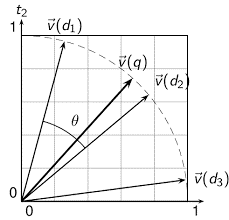
\includegraphics[width = 8cm]{Picture1.png}
	\caption{Vector en un plano}
	\label{fig:plano}
\end{figure}
\begin{figure}[h]
	\center
	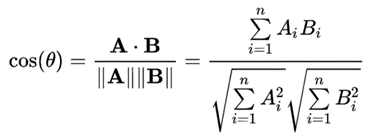
\includegraphics[width = 12cm]{Picture2.png}
	\caption{Fórmula de la similitud del coseno}
	\label{fig:fórmula}
\end{figure}
En este método las variables más importantes que creo son el double [] productoPunto que va a ir guardando la sumatoria de la multiplicación de cada término de la query con el que le corresponde según la posición en la fila de la matriz, el double [] magnitud que guarda la multiplicación de la longitud(raíz cuadrada de la sumatoria de cada término al cuadrado de los vectores que se tienen en cuestión, multiplicación de los módulos de toda la vida) en el espacio de del vector query y el vector del documento correspondiente en la fila de la matriz y el double [] similitud que contiene la división de los arrays antes expuestos.
Luego guardo en la clase Moogle dentro de la clase publica SerchResult una variable similitud asignándole el valor de salida del método SimilitudDelCoseno.
\subsection{Método \texttt{Resultado}}\label{sub:center}
Luego a partir del método Resultado voy a guardar en una variable todos los títulos (ese método utiliza la clase Path para encontrar los títulos de los documentos). Después de eso ordeno los términos de la variable similitud para obtener los scores de mayor a menor y a través del método Snipet tomo un fragmento donde aparezca la palabra con más score de la query.
\subsection{Método \texttt{Levenshtein}}\label{sub:center}
Para crear la sugerencia utilicé el algoritmo de la distancia de Levenshtein adaptado a mi trabajo este está implementado en el método llamado Levenshtein que se basa en encontrar palabras similares a las de la query hallando la palabra de mi lista que necesita la menor cantidad de transformaciones posibles para ser igual a la de mi query. También implemente que si todas las palabras de la query aparecen en mi lista no ponga sugerencia (haciendo uso de arrays de bool) y en el razor cree el método Suggestion que a través del vínculo que otorga la sugerencia pueda realizarse la búsqueda de esta.
\begin{figure}[h]
	\center
	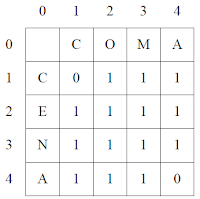
\includegraphics[width = 6cm]{Picture4.png}
	\caption{Matriz de similitud entre palabras}
	\label{fig:levenshtein}
\end{figure}
\newpage
\section{Conclusiones}\label {sec:concl}
Se lograron completar los objetivos del trabajo ya que se aplicaron conocimientos de Álgebra Lineal. La búsqueda a medida q progresaba el proyecto era más rápida y precisa, además de que se complementó el proyecto con mejoras opcionales para aumentar su funcionalidad.
\end{document}
	